%!TEX root = ../template.tex
%%%%%%%%%%%%%%%%%%%%%%%%%%%%%%%%%%%%%%%%%%%%%%%%%%%%%%%%%%%%%%%%%%%%
%% chapter3.tex
%% NOVA thesis document file
%%
%% Chapter with a short latex tutorial and examples
%%%%%%%%%%%%%%%%%%%%%%%%%%%%%%%%%%%%%%%%%%%%%%%%%%%%%%%%%%%%%%%%%%%%

\typeout{NT FILE chapter3.tex}%

\makeatletter
\newcommand{\ntifpkgloaded}{%
  \@ifpackageloaded%
}
\makeatother


\chapter{Experiment}
\label{cha:experiment}

\epigraph{
	"Somewhere, something incredible is waiting to be known."
}{Carl Sagan}



\section{Context and Goal of the Experiment} % (fold)
\label{sec:contex_goal_experiment}

The proposed experiment, detailed in research proposal G-24-00249 \cite{panin2024neutron}, aims to investigate the structure of the neutron-rich fluorine isotope, $^{25}$F, through one-proton knockout reactions. This study is motivated by the "drastic extension of the neutron drip line for Z=9 compared to Z=8 isotopes," a phenomenon that remains poorly understood \cite{ahn_location_2019}. The experiment seeks to elucidate how the $^{24}$O core is polarized by the presence of an additional proton in $^{25}$F, thereby shedding light on the mechanisms responsible for the observed drip line extension.

The experiment will employ the quasi-free scattering (\gls{QFS}) reaction $^{25}$F(p,2p)$^{24}$O in inverse kinematics, effectively knocking out a deeply bound valence proton from the $^{25}$F nucleus \cite{panin_exclusive_2016}. This approach will utilize the \gls{R3B} experimental setup, including the high-efficiency neutron detector NeuLAND \cite{boretzky_neuland_2021}, to achieve complete kinematic measurements and obtain accurate spectroscopic information on the populated final states of $^{24}$O. By analyzing the experimental data, researchers aim to determine the extent to which the single $d_{5/2}$ proton in $^{25}$F modifies the structure of the core nucleons, potentially indicating deformation or polarization of the $^{24}$O core \cite{macchiavelli_core_2020}.

Ultimately, the goal of this experiment is to provide a more detailed understanding of the nuclear structure of neutron-rich fluorine isotopes and the underlying reasons for the extended neutron drip line at Z=9. The results will contribute to a more comprehensive picture of nuclear forces and structure in exotic nuclei, addressing a fundamental question in nuclear physics.


\underline{ADD IMAGE OF ISOTOPE CHART SHOWCASING THE DIFFERENCE IN THE NEUTRON DRIP LINE}


\section{The GSI Accelerator System}
Annex \ref{ann:gsi_facility}

The previously described experiment will take place at the GSI Helmholtzzentrum für Schwerionenforschung in Darmstadt, Germany. GSI’s accelerator complex, seen in Figure \ref{fig:GSI}, provides the infrastructure required to produce and deliver rare isotope beams, such as $^{25}$F, for inverse kinematics reactions. The \gls{R3B} setup, located in Cave C downstream of the FRS, enables complete kinematic reconstruction, making it well-suited for the spectroscopic investigation of exotic nuclei. The following sections outline the accelerator chain that delivers these beams—from ion production through the UNILAC and SIS18 to the FRS and the experimental area.

\begin{figure}
	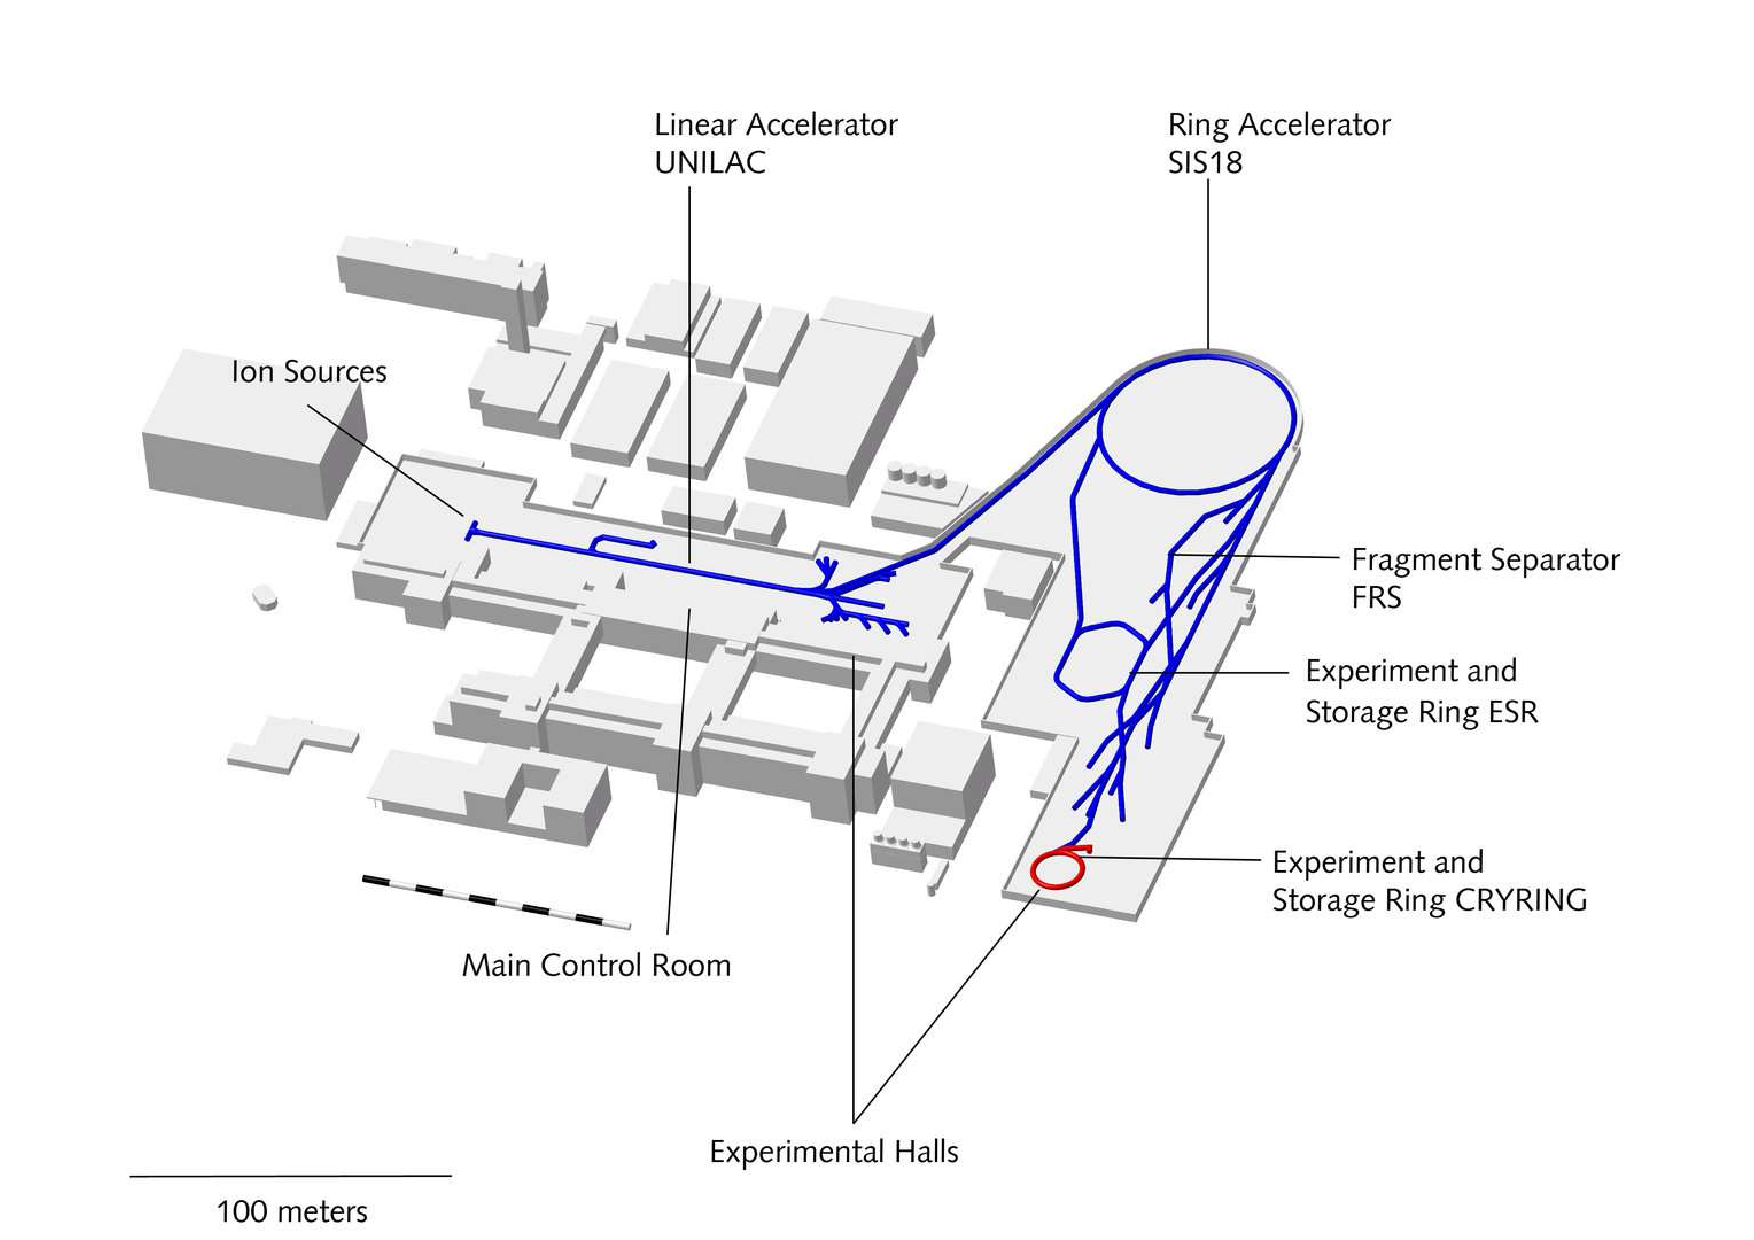
\includegraphics[width=\linewidth]{GSI}
	\caption{Schematic layout of the GSI Helmholtzzentrum accelerator facility. The diagram shows the major components including the ion sources, the UNILAC linear accelerator, the SIS18 synchrotron, the Fragment Separator (FRS), and the associated experimental halls \cite{gsiAcceleratorFacility}.}
	\label{fig:GSI}
\end{figure}


\subsection{From Source to Experimental Cave}

\subsubsection{Ion Production}

The accelerator cycle begins with the production of ions in specialized ion sources. Depending on the experimental requirements, different types of sources are used, including electron cyclotron resonance (ECR) sources and Penning ion sources \cite{hollinger_status_2008}. These generate high charge state ions by stripping electrons from atoms in a plasma environment. The produced ions are pre-accelerated and then injected into the linear accelerator for further acceleration.


\subsubsection{The UNILAC}

The Universal Linear Accelerator (UNILAC) \cite{vormann_high_2023} serves as the primary injector for the GSI accelerator chain. It accelerates ions to energies of several MeV/u before their injection into the synchrotron. Structurally, the UNILAC consists of several stages: a radio-frequency quadrupole (RFQ), an interdigital H-mode drift tube linac (IH-DTL), and a transfer line to the synchrotron SIS18 \cite{barth_high_2022}. Over the years, substantial upgrades have been implemented to accommodate high-intensity beams and improve the beam quality for heavy ion acceleration . The layout of the UNILAC and its role as the front-end of the accelerator chain is depicted in Figure \ref{fig:UNILAC}.


\begin{figure}
	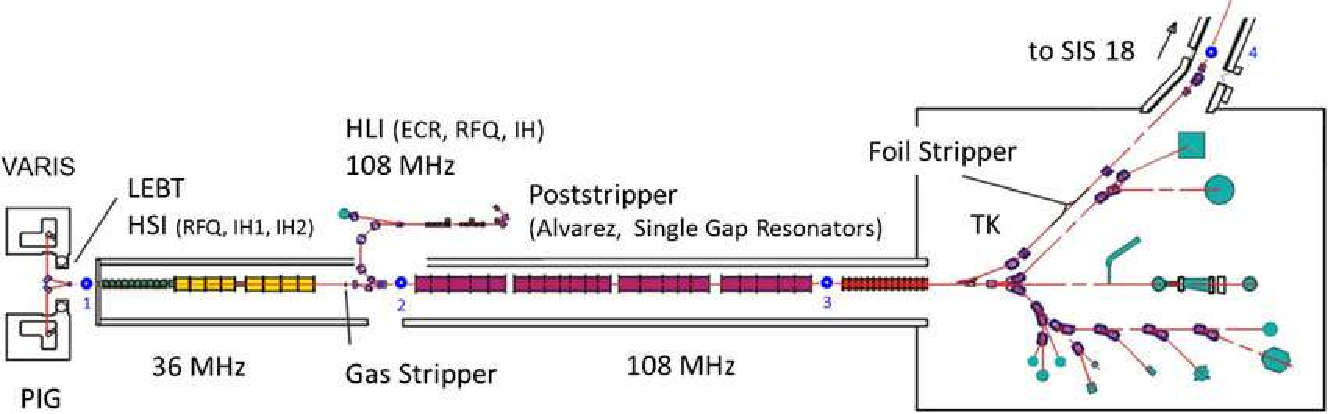
\includegraphics[width=\linewidth]{UNILAC}
	\caption{Detailed schematic of the UNILAC accelerator. The figure highlights the beamline structure from ion sources through the High Current Injector (HSI), Radio-Frequency Quadrupole (RFQ), Interdigital H-mode Drift Tube Linacs (IH-DTL), gas stripper section, Alvarez Drift Tube Linac (DTL), and the transfer line to SIS18. Beam diagnostic and stripping sections are also labeled \cite{barth_high_2022}.}
	\label{fig:UNILAC}
\end{figure}


\subsubsection{The SIS18}

Following pre-acceleration by the UNILAC, ion beams are injected into the SIS18 synchrotron \cite{singh2014tune}, where they are further accelerated to relativistic energies. The SIS18 is a fast-cycling synchrotron with a magnetic rigidity of up to 18 Tm, capable of accelerating ions to several hundred MeV/u. It incorporates sophisticated beam manipulation techniques including bunch compression and multiturn injection to optimize performance and beam delivery. Figure \ref{fig:SIS18} illustrates the SIS18 layout and its specifications. The synchrotron serves both as a terminal accelerator for in-house experiments and as an injector for future FAIR components.

\begin{figure}
	\centering
	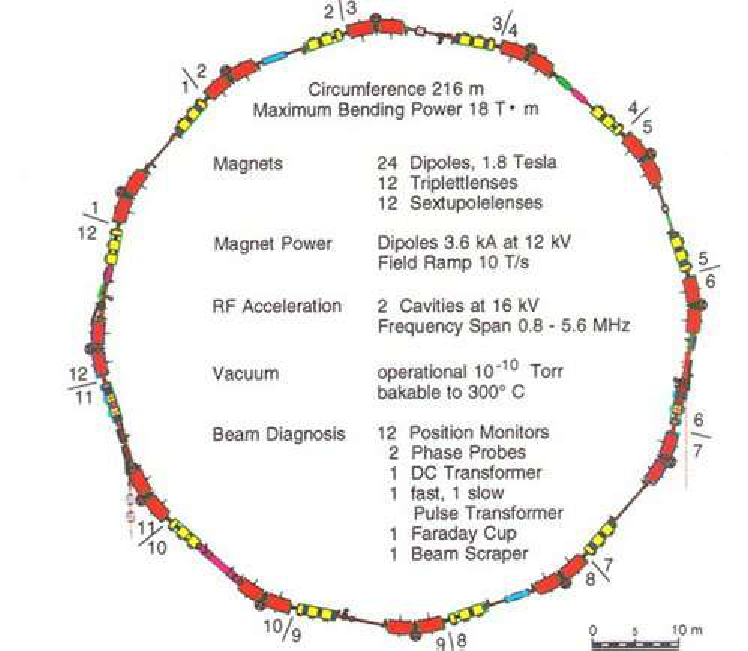
\includegraphics[width=0.7\linewidth]{SIS18}
	\caption{Plan view of the SIS18 heavy-ion synchrotron, illustrating its 12 identical lattice sections, dipole and quadrupole magnet configurations, RF acceleration cavities, and positions of beam diagnostic systems \cite{gsiSIS18Sections}.}
	\label{fig:SIS18}
\end{figure}

\subsubsection{The Fragment Separator (FRS)}

High-energy ions exiting the SIS18 are directed to the \gls{FRS} \cite{geissel_experiments_2008}, a magnetic spectrometer designed for in-flight separation of rare isotopes. The FRS exploits differences in magnetic rigidity and energy loss to isolate specific nuclear species from a cocktail beam. It comprises four dipole magnets forming a two-stage separation system and includes focal planes for tracking, time-of-flight, and energy-loss measurements . As shown in Figure \ref{fig:FRS}, the FRS facilitates beam transport from SIS18 to various experimental areas, enabling studies of exotic nuclei and reaction mechanisms.


\begin{figure}
	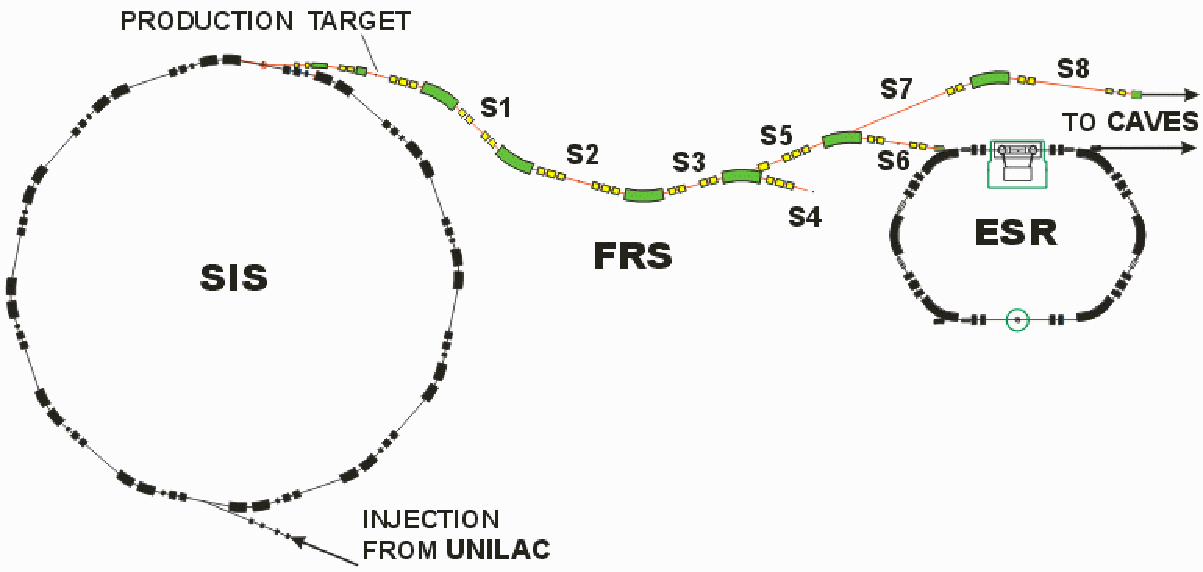
\includegraphics[width=\linewidth]{FRS}
	\caption{Schematic of the FRS system showing its dipole magnet sections, dispersive and achromatic focal planes (F1–F8), and the separation of rare isotope beams. The figure also shows the branching to dedicated experimental areas, including the Direct Branch, Ring Branch (ESR), and the experimental caves \cite{gsiWebHomelt}.}
	\label{fig:FRS}
\end{figure}


\subsubsection{Experimental Caves}

Following separation in the \gls{FRS}, ion beams are directed toward a suite of experimental stations, commonly referred to as experimental caves. These caves are equipped for diverse research programs ranging from nuclear structure and astrophysics to plasma physics and medical applications. One of the principal experimental areas is Cave C, located directly downstream of the FRS. This cave is the one that hosts the \gls{R3B} setup.

Cave C serves as a prototype environment for the future NUSTAR experiments at \gls{FAIR}. Specifically, the \gls{R3B} instrumentation and experimental approach implemented at GSI are being used to develop and validate detector technologies and methodologies for the NUSTAR Cave under construction at \gls{FAIR}. This strategic continuity ensures a seamless transition of experimental capabilities and scientific objectives from the current GSI facility to the \gls{FAIR} complex.

The overall layout of the GSI accelerator chain and its future integration with FAIR, including the locations of Cave C and the planned NUSTAR cave, is illustrated in Figure \ref{fig:GSI_FAIR_R3B}.

\begin{figure}
	\centering
	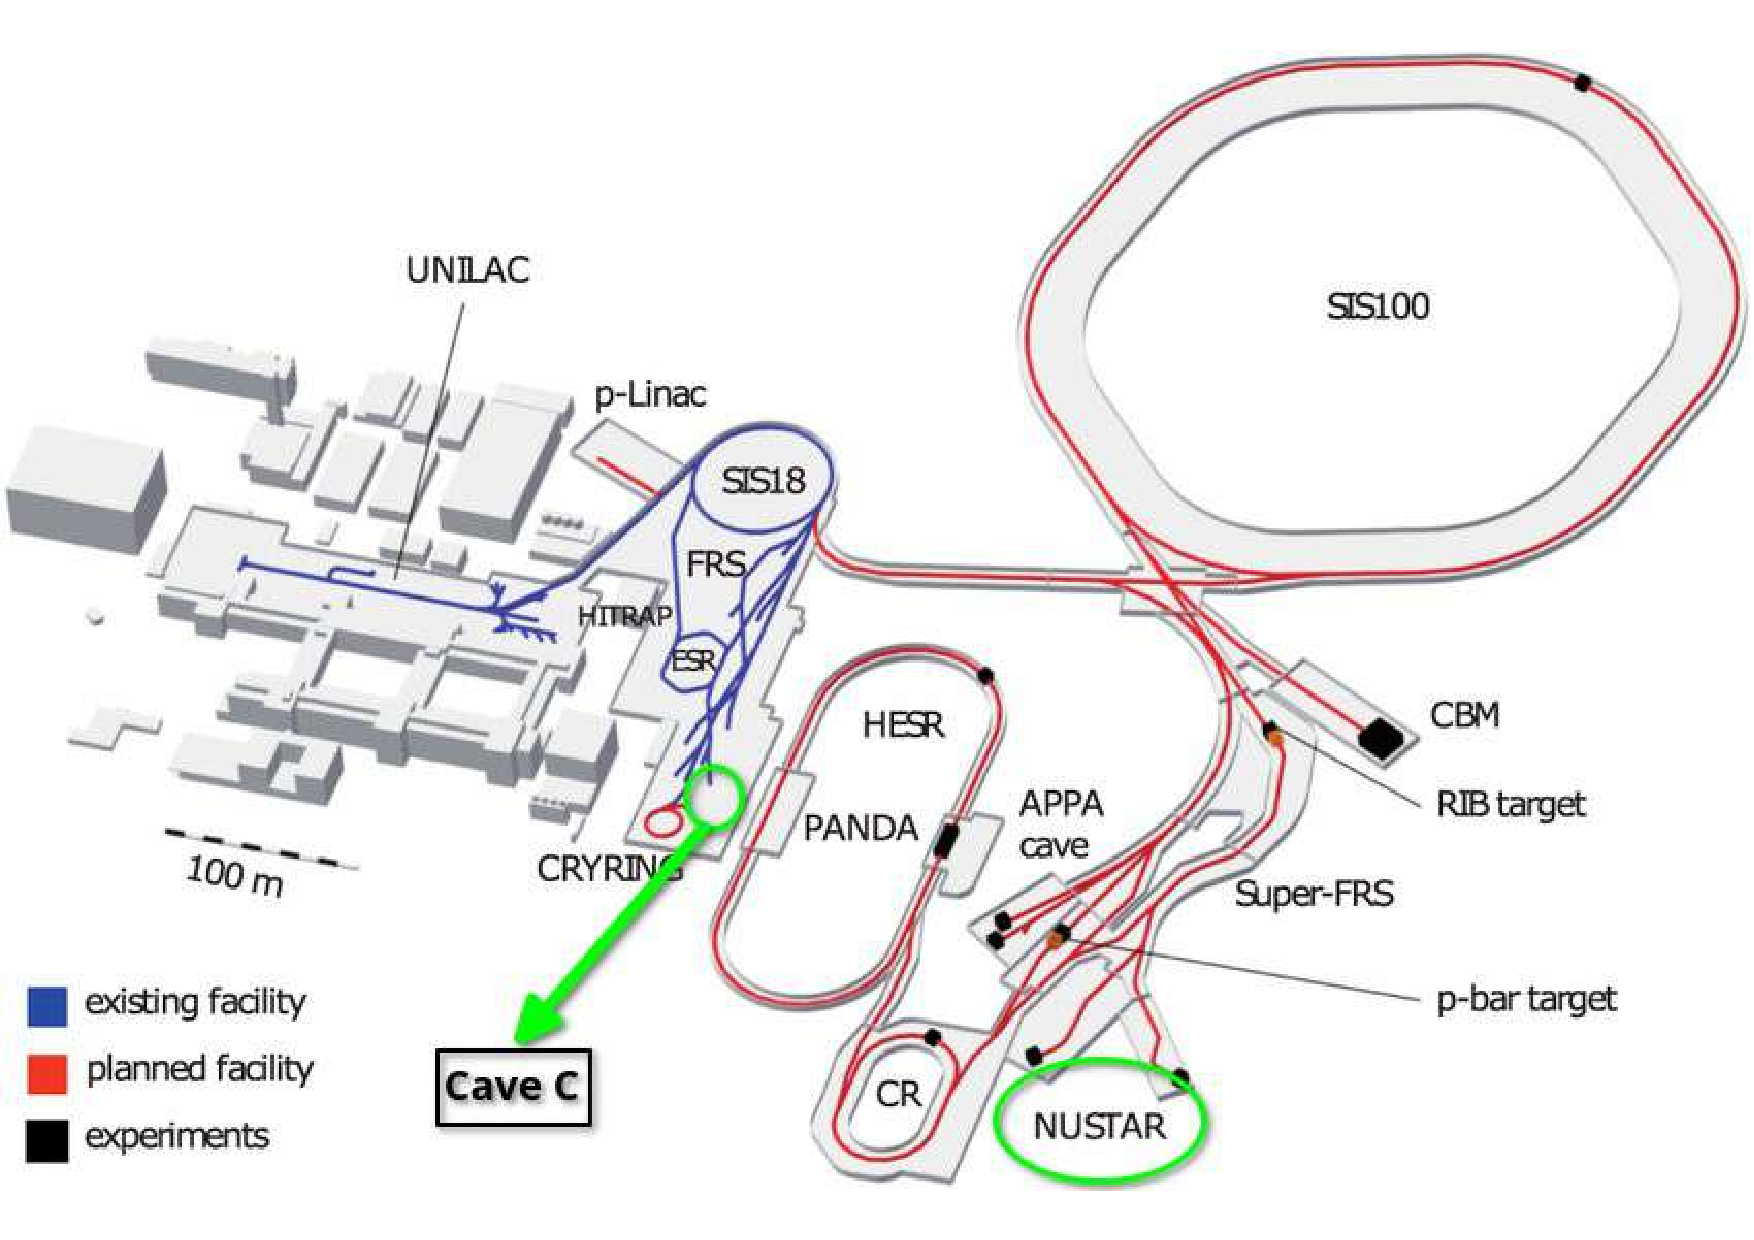
\includegraphics[width=0.8\linewidth]{FAIR_R3B}
	\caption{Layout of GSI-FAIR with Cave C highlighted, where the prototype of the future NUSTAR R$^3$B setup stands and where the present experiment took place.}
	\label{fig:GSI_FAIR_R3B}
\end{figure}


\subsubsection{Summary}

The GSI accelerator system exemplifies a complex yet highly coordinated infrastructure, progressing from ion production through successive acceleration stages and culminating in precision experiments. The integration of the UNILAC, SIS18, and \gls{FRS} ensures the delivery of high-intensity, high-quality ion beams, establishing GSI as a cornerstone of heavy ion research.



\subsection{Beam used in Experiment}

In the proposed experiment \cite{panin2024neutron}, a $^{40}$Ar primary beam with an energy of 700 MeV/u is employed to produce a secondary beam containing the $^{25}$F isotope of interest. The primary beam impinges on a beryllium target located at the \gls{FRS}, inducing nuclear fragmentation reactions. This process generates a cocktail beam consisting of various isotopes, including $^{25}$F, which is then selected and guided towards the experimental setup in Cave C.

The \gls{FRS} is used to separate and purify the secondary beam, ensuring a sufficient intensity of $^{25}$F for the subsequent experiment. As seen in Figure \ref{fig:CocktailBeam}, LISE++ simulations, using the EPAX3.1a production model, predict an intensity of approximately 30 ions per second (pps) of $^{25}$F on the secondary target \cite{panin2024neutron}. The total intensity of the secondary cocktail beam in Cave C is expected to be below 700 pps, with a purity of around 5\% for $^{25}$F \cite{panin2024neutron}. The relatively low total intensity allows for data acquisition without significant downscaling of triggers and minimizes dead time.

In Cave C, the $^{25}$F secondary beam interacts with a liquid hydrogen (LH2) target, which serves as the reaction target for the one-proton knockout reaction $^{25}$F(p,2p)$^{24}$O. The LH2 target is positioned in the center of the CALIFA calorimeter, enabling the detection of outgoing protons from the reaction. The use of a 150 mm thick LH2 cell was initially planned but, due to problems in the liquefaction phase, the cell was replaced for a 50 mm one, reducing the reaction yield. 

%The use of a 150 mm thick LH2 cell maximizes the reaction yield, compensating for the low intensity of the $^{25}$F beam.

\begin{figure}
	\centering
	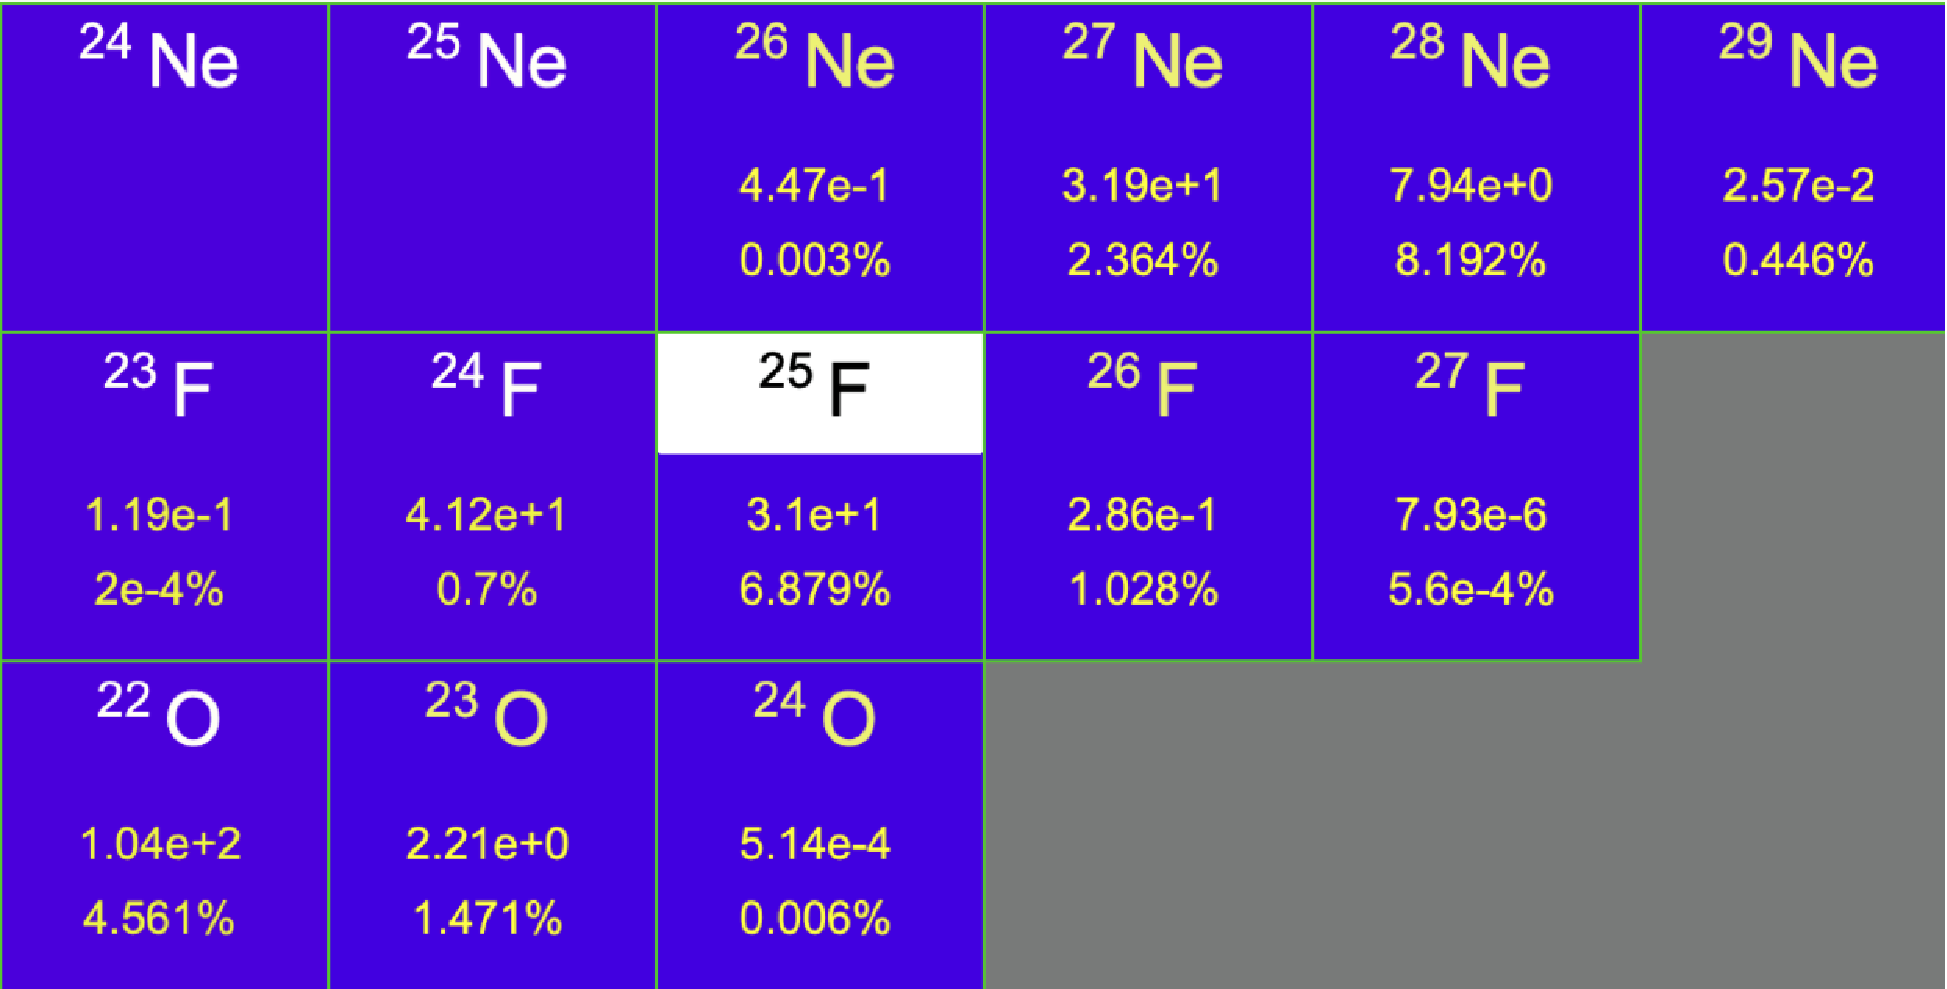
\includegraphics[width=0.75\linewidth]{CocktailBeam}
	\caption{Expected secondary cocktail beam of $^{25}$F in Cave C as obtained by LISE++ calculations. The numbers under the names of isotopes indicate calculated rates per second. Reprinted figure from Ref. \cite{panin2024neutron}.}
	\label{fig:CocktailBeam}
\end{figure}


\section{R$^3$B Setup}

%The \gls{R3B} (Reactions with Relativistic Radioactive Beams) experimental setup at GSI is designed for kinematically complete measurements of nuclear reactions involving fast exotic beams. It integrates a series of tracking and particle-identification detectors, calorimeters, spectrometers, and neutron detectors. In the present experiment, the detectors are arranged along the beamline to capture the full final-state topology of the quasi-free scattering reaction $^{25}$F(p,2p)$^{24}$O, allowing precise reconstruction of reaction kinematics and spectroscopy of the residual nucleus.

The \gls{R3B} (Reactions with Relativistic Radioactive Beams) setup at GSI is designed for high-precision, kinematically complete measurements of nuclear reactions involving rare isotope beams at relativistic energies. For the investigation of the $^{25}$F(p,2p)$^{24}$O reaction, the configuration is optimized to detect all relevant particles emerging from the target—charged fragments, recoil protons, and neutrons—with high resolution and full angular coverage. The following description reflects the actual experimental layout, based on the schematic shown in Figure \ref{fig:ExperimentalSetupSketch}, and supported by the experimental proposal and detector-specific references.

\begin{figure}
	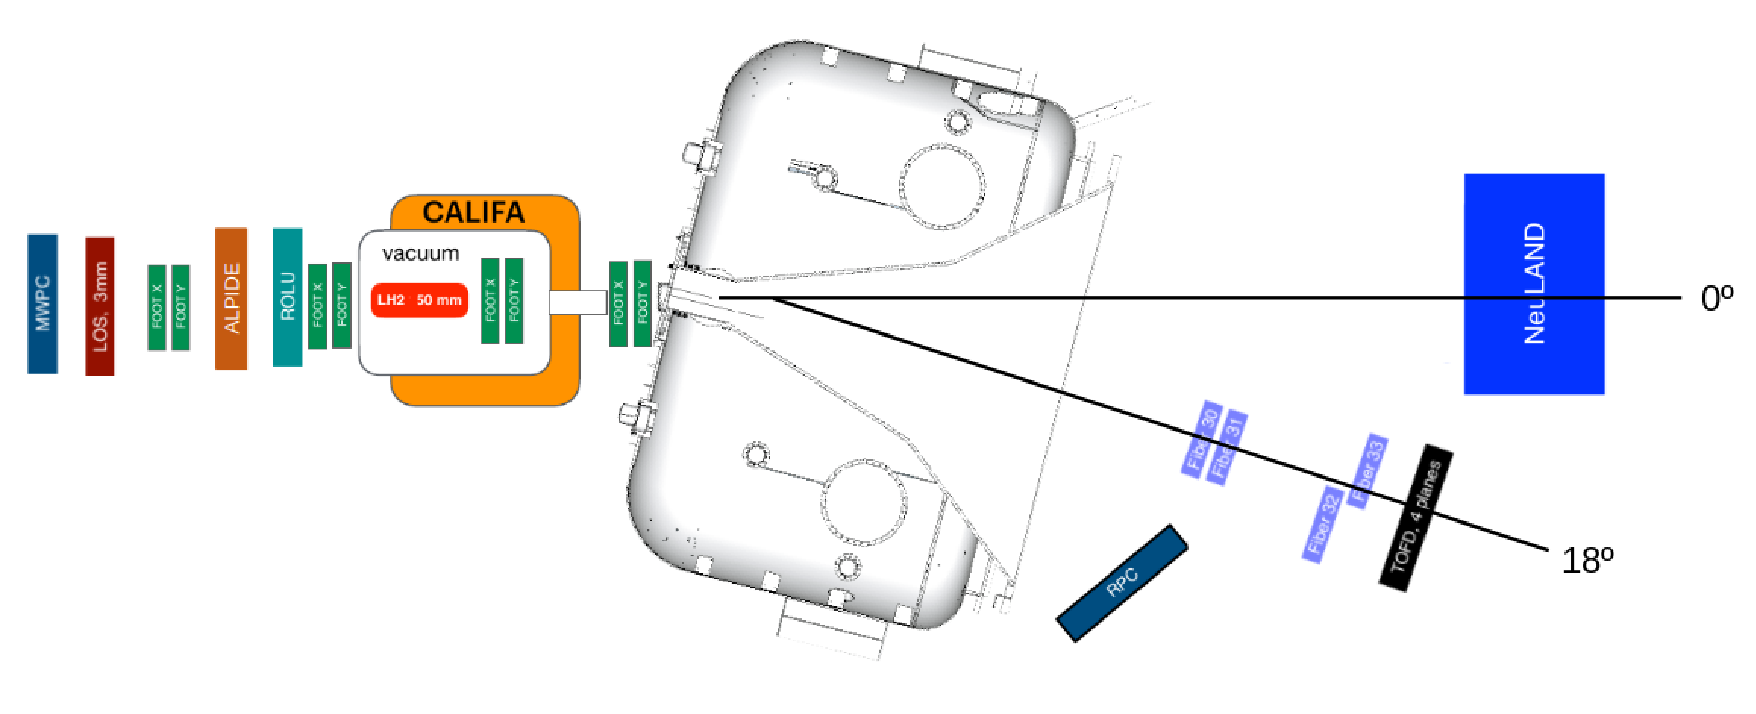
\includegraphics[width=\linewidth]{ExperimentalSetupSketch}
	\caption{Sketch of the experimental setup at R$^3$B.} %Reprinted figure from Ref. \cite{panin2024neutron}.}
	\label{fig:ExperimentalSetupSketch}
\end{figure}

\begin{figure}
	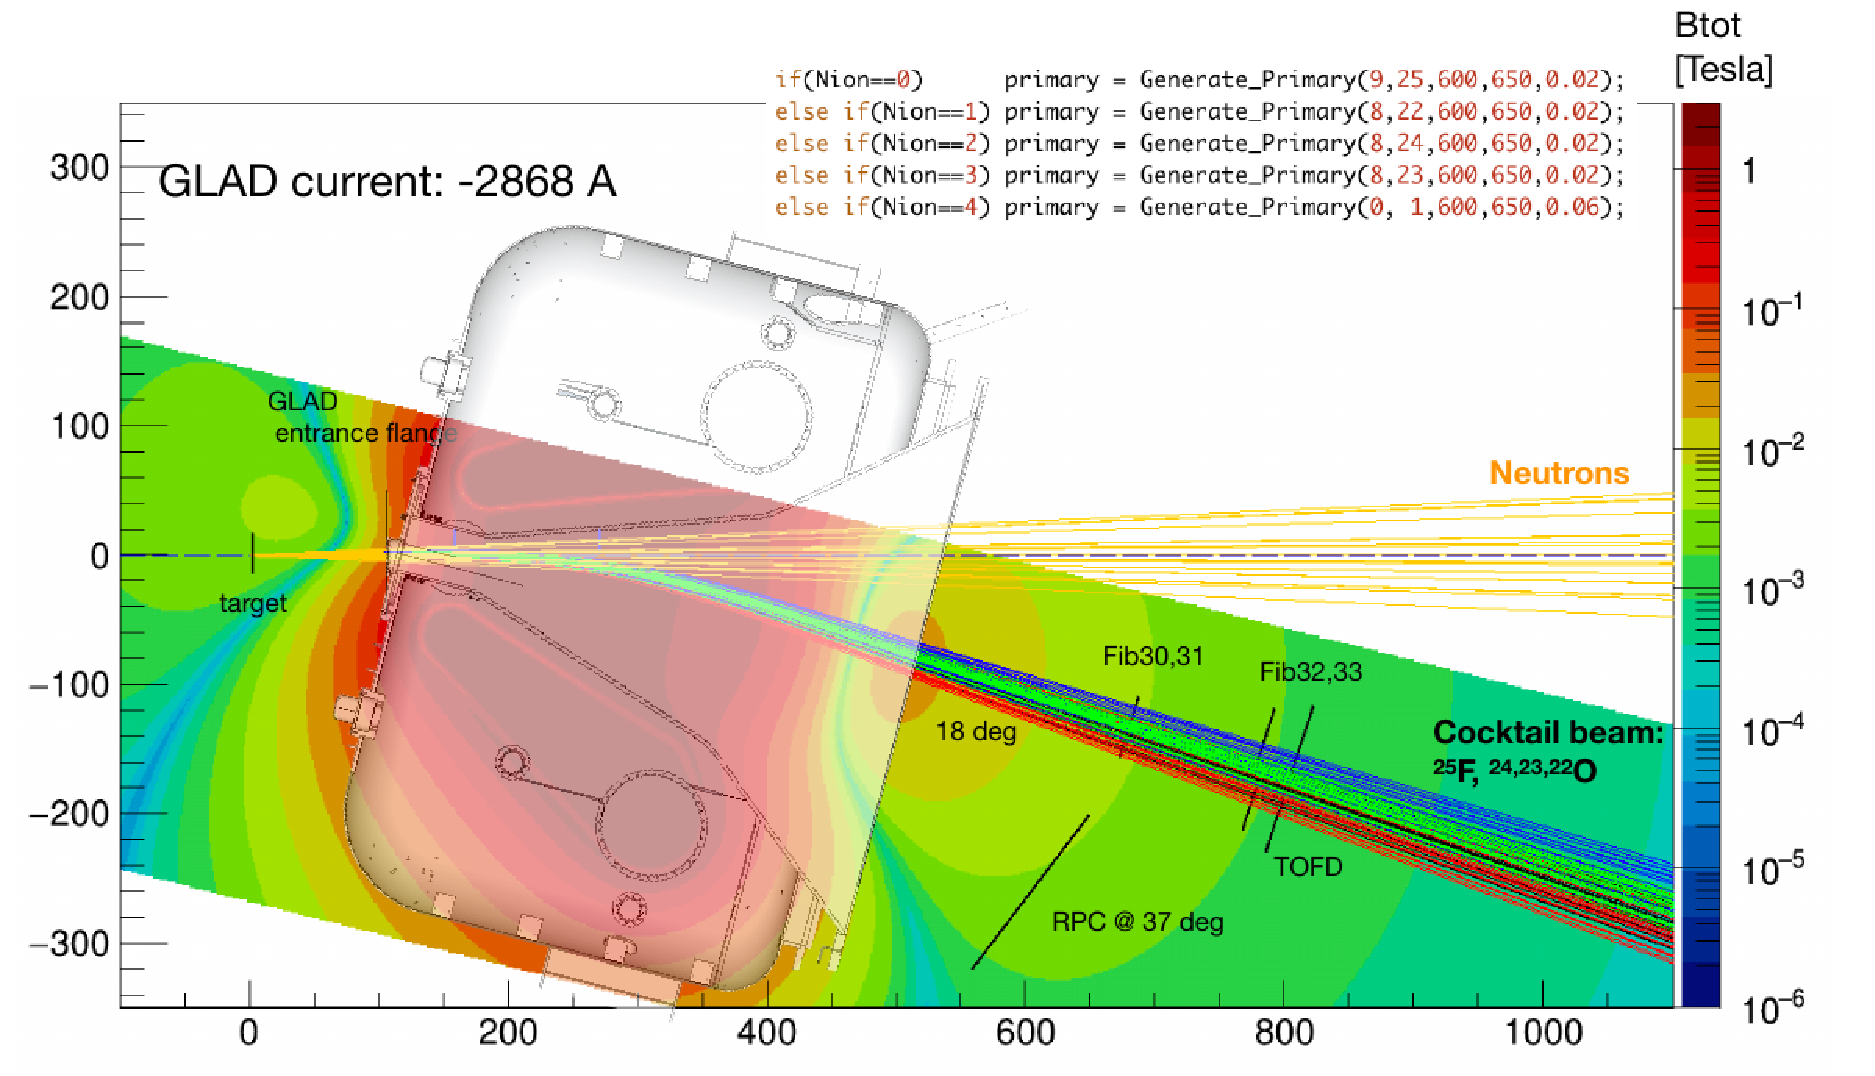
\includegraphics[width=\linewidth]{TrajectorySimulations}
	\caption{Simulated trajectories through the GLAD magnet. The color map indicates the magnetic
		field of the magnet. The LH2 target is located at the (0,0,0) point in front of GLAD. Reprinted figure from Ref. \cite{panin2024neutron}.}
	\label{fig:TrajectorySimulations}
\end{figure}



\begin{newpdflayout}{210mm}{297mm}%{420mm}
	
	\begin{figure}
		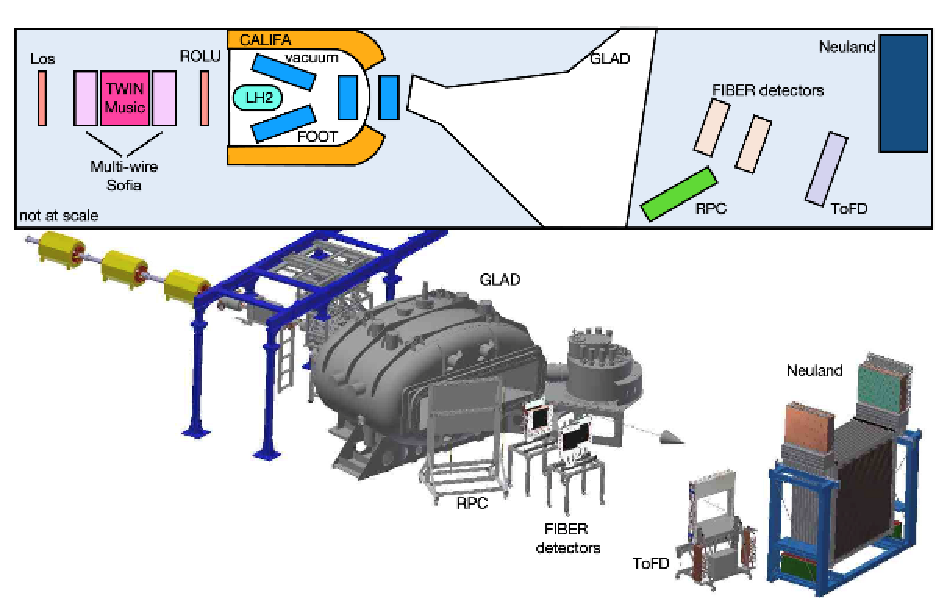
\includegraphics[width=\linewidth]{R3BSetup}
		\caption{}
		\label{fig:R3B_Setup}
	\end{figure}

\end{newpdflayout}

\gls{R3B}

\gls{R3B}

\gls{ToFD}

\gls{ToFD}

\gls{NeuLAND}

\gls{NeuLAND}

\gls{GLAD}

\gls{GLAD}

\gls{CALIFA}

\gls{CALIFA}

\gls{RPC}

\gls{RPC}
\begin{figure}
	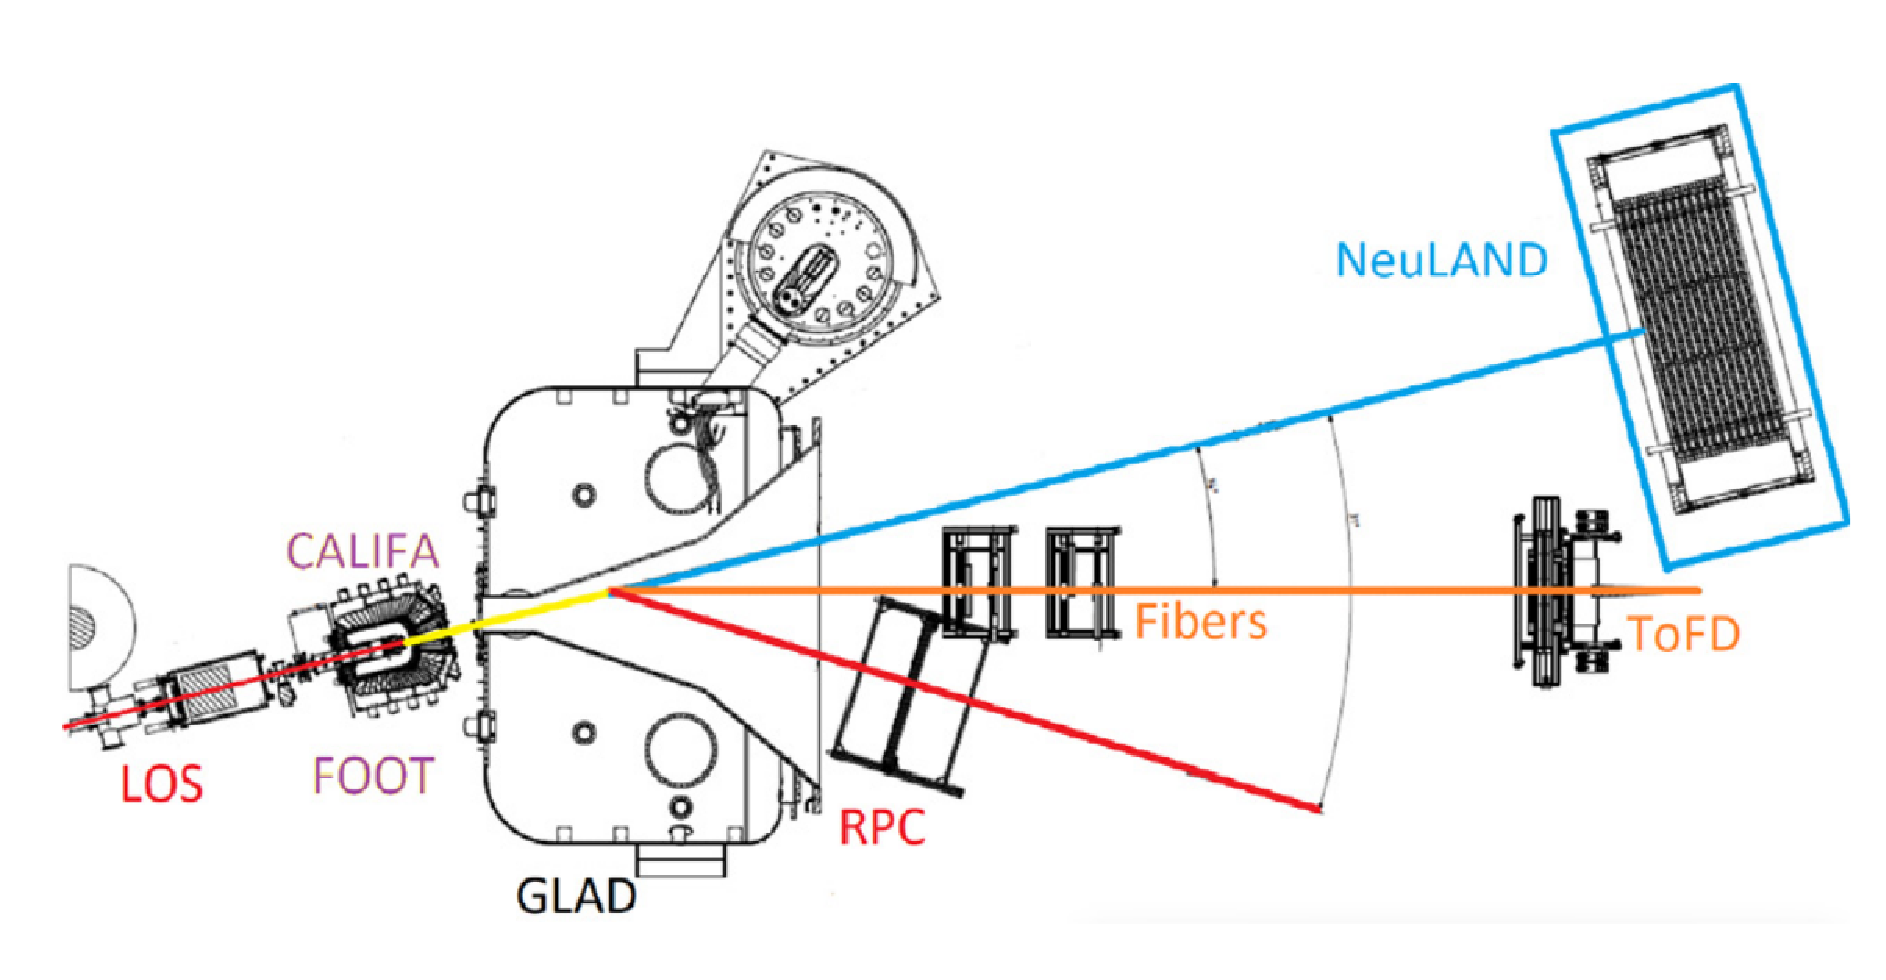
\includegraphics[width=\linewidth]{SchematicR3BSetup}
	\caption{Schematic representation of the R$^3$B setup with beam lines.}
	\label{fig:R3BSetup}
\end{figure}



\subsection{Role of each detector}

ALPIDE \cite{mager_alpide_2016}.

\subsubsection{Incoming Beam Tracking and Identification}

The secondary beam of $^{25}$F enters the experimental area and is tracked and identified using a series of detectors placed along the beamline. The first two components, \textbf{MWPC0} and \textbf{MWPC1}, are multi-wire proportional chambers that provide precise position and angular information of the incoming ions with minimal material budget. This tracking is essential for reconstructing the reaction vertex within the extended target and for correlating the incoming ion with its downstream reaction products \cite{paschalis_-beam_2015}.

Following these are the \textbf{TwinMUSIC} chambers, a dual-section ionization detector that measures the energy loss ($\Delta$E) of incoming particles to determine their nuclear charge (Z). This is especially important in purifying the cocktail beam and identifying the rare $^{25}$F ions on an event-by-event basis.

Immediately downstream of TwinMUSIC is the \textbf{LOS} (Large-area Organic Scintillator), which functions as the start detector for time-of-flight (ToF) measurements and provides an additional layer of Z identification via fast plastic scintillation. It also contributes to triggering logic for reaction events \cite{panin2024neutron}.

The final upstream detector before the target is \textbf{ROLU}, a collimating slit used to define the spatial beam profile and eliminate halo components. While not used for measurement directly, it is essential for ensuring clean beam passage into the reaction chamber.


\subsubsection{Target Region}

The nuclear reaction takes place inside a 50 mm liquid hydrogen (LH$_2$) target, located at the center of the setup. This thick cryogenic target is ideal for maximizing reaction yields in low-intensity beams, especially for quasi-free scattering processes like (p,2p) in inverse kinematics. The outgoing protons and reaction residues emerge from the target into a nearly 4$\pi$ detection environment.

Surrounding the target is \textbf{CALIFA} (CALorimeter for In-Flight particles and $\gamma$-rays), a highly segmented electromagnetic calorimeter composed of CsI(Tl) crystals. CALIFA plays a dual role: it detects prompt $\gamma$-rays from de-exciting nuclei and captures recoil protons from the (p,2p) process. Its barrel geometry provides angular resolution suitable for identifying proton pairs and determining their opening angles, which are key to selecting quasi-free events. The energy resolution is approximately 5–6\% at 1 MeV, and the time resolution is sub-nanosecond, enabling precise event reconstruction \cite{cortina-gil_califa_2014}.


\subsubsection{Fragment Tracking Before and After the Magnet}

Charged reaction fragments are tracked using \textbf{FOOTs} (Fast Outgoing Object Trackers), which are double-sided silicon-strip detectors. The first pair of FOOTs (X and Y planes) is positioned directly downstream of the target, inside the CALIFA chamber, while the second pair is located just after CALIFA. These detectors provide position, angle, and energy-loss measurements, facilitating both trajectory reconstruction and Z identification of heavy residues such as $^{24}$O, $^{23}$O, and $^{22}$O \cite{panin2024neutron}.


\subsubsection{Magnetic Analysis with GLAD}

After exiting CALIFA and the second FOOT pair, the charged fragments enter the field of \textbf{GLAD} (GSI Large Acceptance Dipole), a superconducting dipole magnet with a large aperture and strong bending power (up to 1.6 T·m). In this experiment, GLAD is operated at approximately 58\% of its maximum field, providing sufficient magnetic rigidity to separate fragments by momentum and charge state. This is critical for enabling invariant-mass spectroscopy when combined with tracking and time-of-flight measurements.


\subsubsection{Downstream Fragment Tracking and Identification}

Charged fragments deflected by GLAD are further tracked by \textbf{MWPC3}, a large-area proportional chamber providing coarse but wide-angle position measurements. This is followed by two layers of scintillating fiber detectors, which deliver fine spatial resolution (~100 $\mu$m) for trajectory reconstruction and angular correlation. These tracking elements allow for precise determination of deflection angles, and thus of the total momentum vectors of the reaction products.

At the far end of the fragment line is the \textbf{ToFD} (Time-of-Flight Detector), a large-area plastic scintillator wall composed of four vertical planes. ToFD measures both ToF and energy loss with high precision, achieving timing resolutions of approximately 14 ps per plane and $\Delta$E resolution better than 1\% for Z determination. This data, combined with magnetic rigidity and tracking information, enables full fragment identification in both charge and mass number \cite{heil_new_2022}.

\subsubsection{Neutron Detection with NeuLAND}

Neutral particles emitted in the reaction, primarily neutrons from unbound states of $^{24}$O and lighter oxygen isotopes, travel unaffected by GLAD’s magnetic field and continue on a straight path to the \textbf{NeuLAND} (New Large-Area Neutron Detector). NeuLAND is composed of 3000 plastic scintillator bars arranged in 30 double planes, positioned approximately 15–35 meters downstream of the target at zero degrees. It is optimized for detecting fast neutrons (100–1000 MeV) with high efficiency (93–95\% for single neutrons) and excellent spatial (~1.5 cm) and timing (<150 ps) resolution \cite{boretzky_neuland_2021}.

NeuLAND enables measurement of multi-neutron events (e.g., $^{23}$O + n, $^{22}$O + 2n) via time-of-flight and interaction point reconstruction, and is critical for the invariant-mass reconstruction of the unbound final states populated in the (p,2p) reaction. This functionality allows the extraction of excitation energies and decay modes of exotic oxygen isotopes with unprecedented precision.


\subsection{Particular Role of RPC}

\cite{xarepe_resistive_2023}


\subsection{Main DAQ}

Each detector is connected to the main \gls{DAQ}, everytime they have a trigger, they send a trigger request to the main \gls{DAQ}. If multiple detectors send a trigger request, it is considered an event to register and the main \gls{DAQ} sends an accept signal, allowing every detector to save that signal.

All of these saved signals of each detector are then saved in a common \textit{lmd} file containing every detectors data separated by event.

There's a synchronization signal with around 10 Hz to make sure every detector is synchronized.


\section{Personal Contribution to the Experiment}